% Chapter 1
\chapter{Généralités sur la segmentation de texture} % Main chapter title

\label{Chapter1} % Change X to a consecutive number; for referencing this chapter elsewhere, use \ref{ChapterX}

\lhead{Chapitre 1. \emph{Généralités sur la segmentation de texture}} % Change X to a consecutive number; this is for the header on each page - perhaps a shortened title


\section{introduction}

Dans ce chapitre, nous examinerons les différentes définitions de texture proposés par plusieurs chercheurs du domaine. Puis nous verrons les notions de bases du traitement d'images et un apperçu de ses domaines d'utilisation . Nous découvrirons enfin, plus en détails, la méthodes que nous avons utilisés pour caractériser une textures.

\section{Définition de la texture}

\indent Certaines définitions de la texture ont été sélectionées et regroupées dans un catalogue par Coggins [COG 82]. On peut en citer quelques exemples:\\


\begin{itemize}
\item \indent "Nous pouvons considérer une texture comme ce qui constitue une région macroscopique. Sa structure est simplement attribuable aux motifs répétitifs dans lesquels des éléments ou des primitives sont disposées selon une règle de placement."[Tam et.al 78] \\ 

\item \indent "La texture est défini pour nos fins comme un attribut d'un domaine n'ayant aucune composante qui apparaissent dénombrable. Les relations de phase entre les composants ne sont donc pas apparentes. Le terrain ne devrait pas contenir un gradient évident. Le but de cette définition est d'attirer l'attention de l'observateur sur les propriétés globales de l'affichage -. C'est à dire sa "rudesse" globale "bosselage", ou "finesse". Physiquement, les modèles innombrables (apériodiques) sont générés par stochastique par opposition de processus déterministes. A la perception, cependant, l'ensemble des motifs sans composants énumérables évidentes comprendra de nombreux (et même périodique) textures déterministes."[Ric et.al 74]\\

\item \indent "La texture est une notion apparemment paradoxale. D'une part, elle est couramment utilisée dans le traitement de l'information visuelle, surtout pour des raisons pratiques de classification. D'autre part, personne n'a réussi à produire une définition communément acceptée de la texture. La résolution de ce paradoxe, dépendra d'un modèle plus riche, plus développé pour le début de traitement de l'information visuelle, un aspect central de ce qui sera un systèmes représentatif à différents niveaux d'abstraction. Ces niveaux vont probablement inclure
-----------------------------------------
 intensités actuels au fond et progresseront à travers des pointes et des descripteurs d’orientation vers la surface, et peut-être des descripteurs volumétriques. Compte tenu de ces structures multi-niveaux, il semble clair qu'ils doivent être inclus dans la définition, et dans le calcul des  descripteurs de la texture."[Zuc et.al 81]\\

\item \indent "La notion de texture semble dépendre de trois ingrédients: (1) un certains « ordre » local répété sur une région qui est grande par rapport à la taille de l'ordre, (2) l'ordre consiste en l'arrangement non aléatoire de pièces élémentaires et (3) les parties sont des entités plus ou moins uniformes ayant approximativement les mêmes dimensions partout dans la région texturée."[Haw 69]\\\\
\end{itemize}

\begin{figure}[htbp]
\centering
\begin{tabular}{cc}
\centering
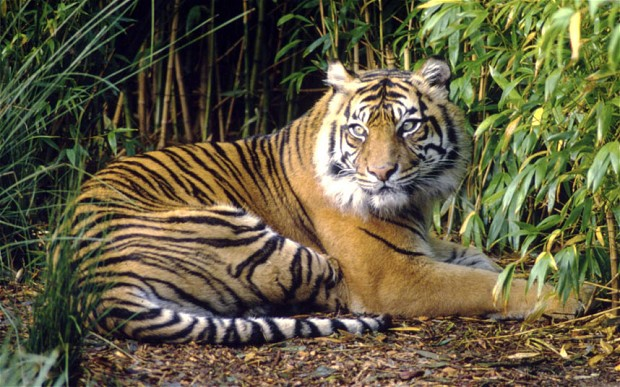
\includegraphics[width=6cm, height=4.5cm]{Figures/chap1/tigre.jpg}
&
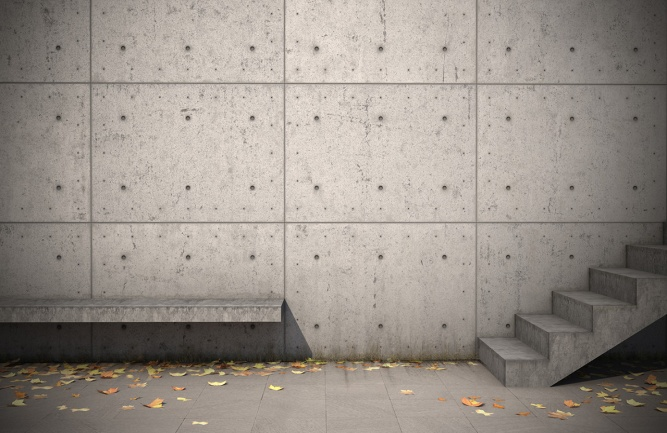
\includegraphics[width=6cm, height=4.5cm]{Figures/chap1/beton.jpg}\\

(a)
 &
(b)

\end{tabular}
\caption[textureDif]{Différentes textures\\}
\end{figure}


Quelques paramètres essentiels sont à prendre en compte dans l’étude des textures. Si on prend par exemple la photo d’une forêt, on pourra distinguer la terre comme texture,  l’ensemble des feuille d’un arbre comme une autre, mais encore la peau d’un tigre [Figure 1.1](a).\\

Si on prend par contre une prise aérienne de cette même forêt, on pourra considérer le tout comme une seule texture qui se différenciera de la texture formée par les bâtiments d’un village par exemple. 
Aussi, le voisinage d’une texture joue un grand rôle dans l’interprétation de cette dernière. Une couche de béton par exemple seule peut avoir plusieurs interprétations, elle peut être une partie d’un mur,  un banc, le sol ou  bien des marches d’escalier [Figure 1.1](b).\\

Notons aussi que certaines structures ont une dynamique importante au fil du temps qui fait varier leur apparence. Par exemple un ciel bleu avec quelques nuages (le vent fera constamment varier la forme des nuages).\\ 

%------------------------------------------------
%-------- [1] SEGMENTATION D'IMAGES -------------
%------------------------------------------------


\section{Segmentation d’images}

\indent Dans le traitement d’image, une des plus grandes préoccupations est la segmentation d’images. C’est, comme son nom l’indique, le processus de partitionnement d’image digitale en différentes parties et ce, pour simplifier la « compréhension »  de cette dernière par la machine, et la rendre plus facilement analysable.\\

Le principe est de reconnaître des objets ou des frontières. Le but étant de donner une signification aux pixels de l’image. Elle est généralement utilisée dans:.\\

\begin{itemize}
\item La vision artificielle [Figure 1.2](a)\\
\item \indent L’imagerie médicale [Figure 1.2](b)\\
\item \indent La reconnaissance faciale [Figure 1.2](c)\\
\item \indent La reconnaissance d'empreintes digitales [Figure 1.2](d)\\
\item \indent La détection de piétons [Figure 1.2](e)\\
\item \indent La vidéo surveillance [Figure 1.2](f)\\
\item \indent Localiser des objets dans des images satellitaires [Figure 1.2](g)\\
\end{itemize}

\begin{figure}[h]
\centering

\begin{tabular}{cccc}

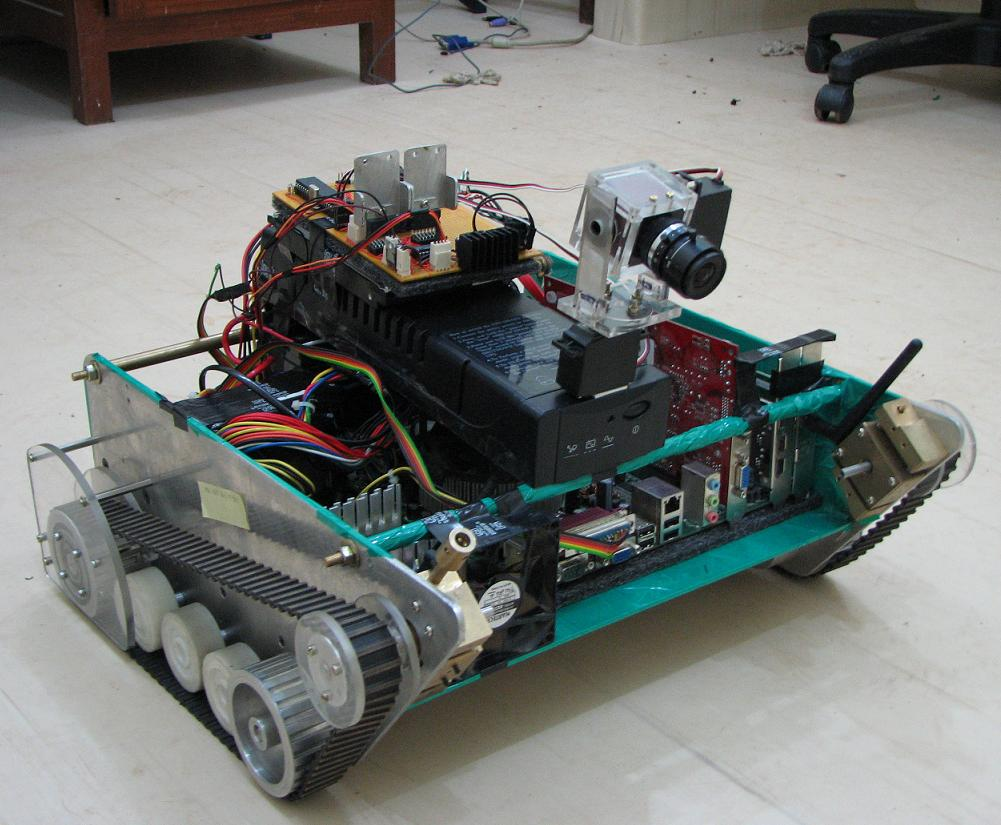
\includegraphics[width=5.5cm, height=3.5cm]{Figures/chap1/VisionArtificielle1.jpg}
&
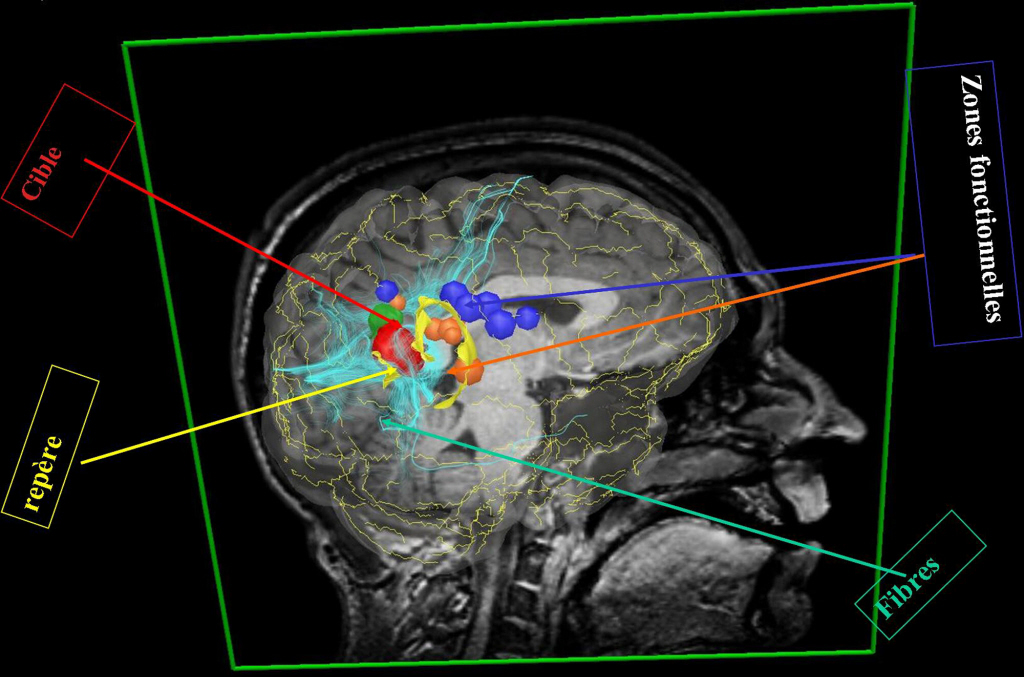
\includegraphics[width=5.5cm, height=3.5cm]{Figures/chap1/ImagerieMedical.jpeg}\\
(a) & (b)\\\\

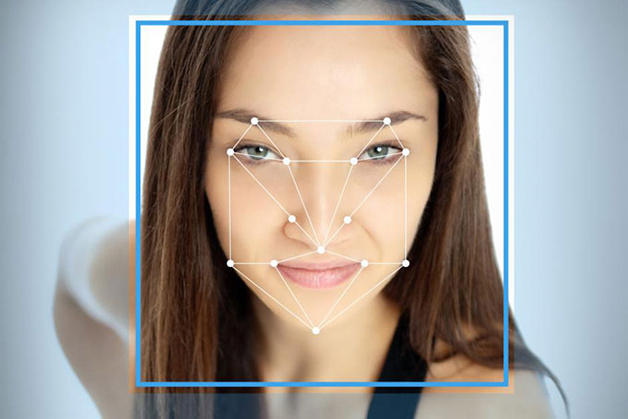
\includegraphics[width=5.5cm, height=3.5cm]{Figures/chap1/reconaissanceFacial.jpg}
&

\includegraphics[width=5.5cm, height=3.5cm]{Figures/chap1/empreinteDigitale.jpeg}\\
(c) & (d)\\\\

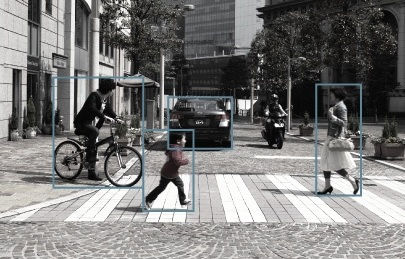
\includegraphics[width=5.5cm, height=3.5cm]{Figures/chap1/DetectionPieton.png}
&
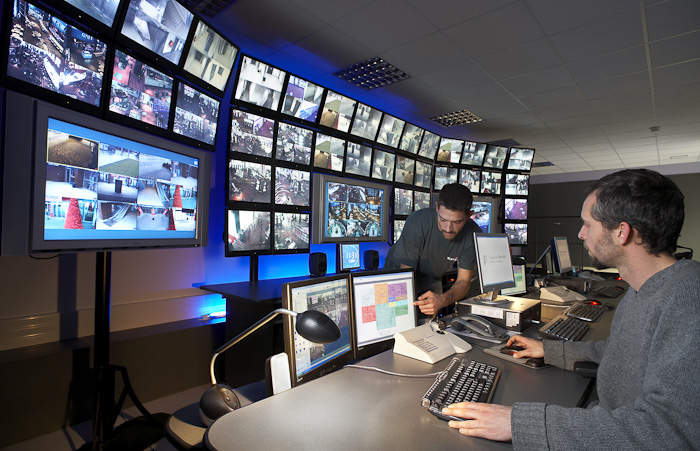
\includegraphics[width=5.5cm, height=3.5cm]{Figures/chap1/videoSurveil.jpeg}\\
(e) & (f)\\\\

\multicolumn{2}{c}{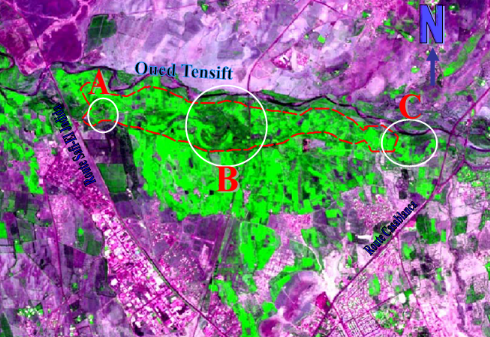
\includegraphics[width=5.5cm, height=3.5cm]{Figures/chap1/Satellite.png}}\\
\multicolumn{2}{c}{(g)}\\

\end{tabular}
\caption[TraitementImage]{La segmentation d'images}

\end{figure}


%------------------------------------------------
%------- [2] LES APPROCHES ANALYTIQUES ----------
%------------------------------------------------

\section{Les approches analytiques}

\indent On retrouve principalement quatre (4) approches analytiques de texture qui sont [MAT et STR 98]:\\
\begin{itemize}
\item \textit{Approche structurelle (ou fréquentielle)}: Ces méthodes supposent que les textures sont formées d’éléments structurants de base. L’idée générale de ces méthodes est une recherche et une description des éléments structurants suivie d’une étude de la répartition spatiale de ces derniers [MAJ 09].\\

\item \textit{Approche modèle} : Elle se repose sur l’utilisation de fractals et de modèles stochastique.\\

\item \textit{Approche transformée (méthodes de traitement du signale)} : Des recherches de  psychophysique ont démontrés que le cerveau humain fait une analyse de fréquence des images.\\ 

\item \textit{Approche statistique} : Ici, la texture est reconnu en utilisant des caractéristique tel que les "\textit{Motifs Binaires Locaux}"  en se basant sur distribution des niveaux de gris dans l’image, et c’est sur quoi sera basée notre approche.\\
\end{itemize}

L’utilisation de ces approches diffère selon le type de texture. Ces dernières se regroupent en trois différentes catégories : structurelles, aléatoires et directionnelles.


\subsection{Textures structurelles}

\begin{figure}[htbp]
\centering
\begin{tabular}{cc}
\centering

	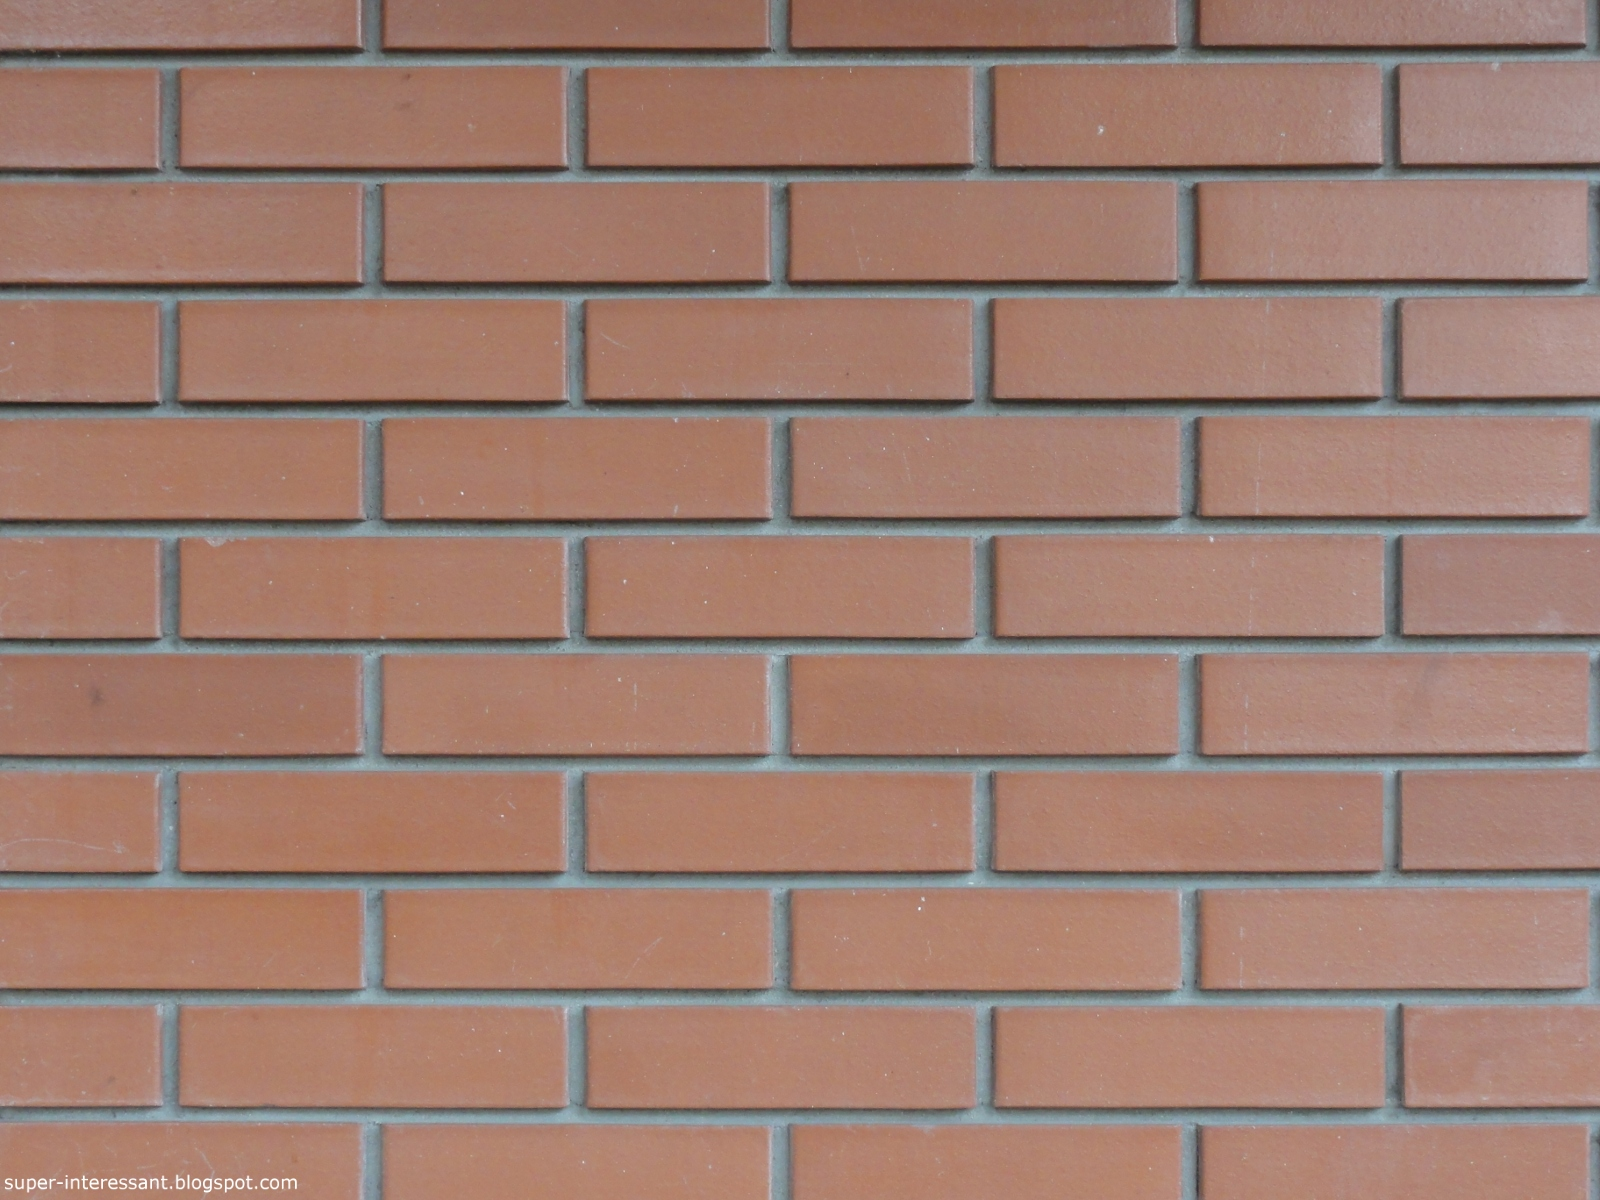
\includegraphics[width=5cm,height=3cm]{Figures/chap1/mur.jpg}	
&
	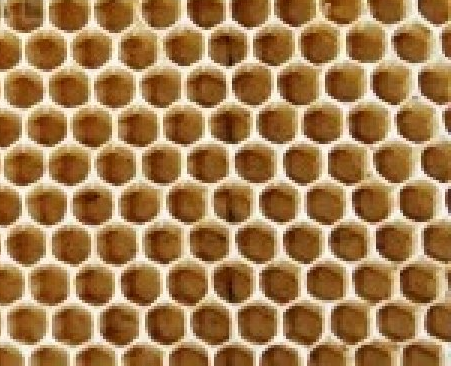
\includegraphics[width=5cm,height=3cm]{Figures/chap1/beehive.png}	

\end{tabular}
	\caption[textureStruc]{Textures structurelles (périodique)}
\label{fig:textureStruc}
\end{figure}


\indent La figure 1.3 présente un premier type de textures dites structurelles.
On les appelle ainsi car on peut les considérer comme étant la répartition spatiale de motifs élémentaires de base dans différentes directions de l’espace tout en respectant une certaine règle de placement. En effet, on s’aperçoit que la première représente un mur de brique, elle est composée d’un ensemble d’éléments de base (les briques) disposés relativement régulièrement de manière horizontale. La deuxième texture est aussi composée de motifs de base alvéolés agencés d’une manière particulière les uns à côté des autres [MAJ 09].
Cette catégorie de textures a engendré des méthodes d’analyse dites structurelles.

\subsection{Textures aléatoires}

\begin{figure}[H]
\centering
\begin{tabular}{cc}
\centering

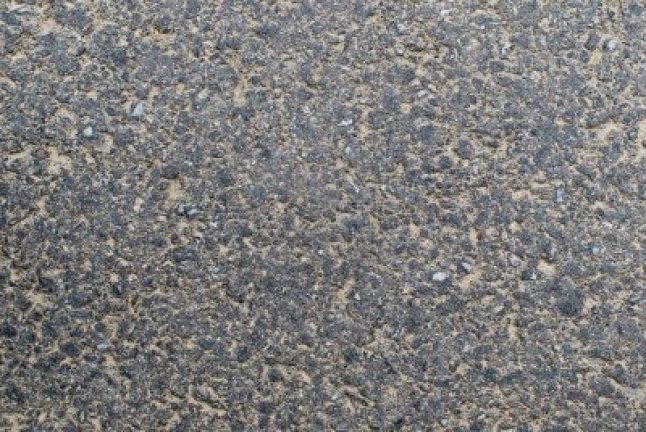
\includegraphics[width=5cm,]{Figures/chap1/aleatoire1.png}
&
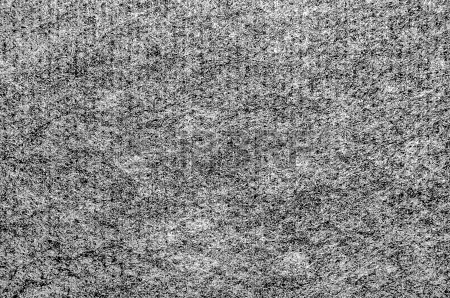
\includegraphics[width=5cm,]{Figures/chap1/aleatoire2.png}\\

\end{tabular}
\caption[textureAleat]{Textures aléatoires}
\end{figure}


\indent Le deuxième type de textures est illustré dans la figure 1.4. Contrairement au premier type de texture, celles-ci ont un aspect anarchique tout en restant globalement homogènes. Ces textures ne peuvent pas être décomposé en des motifs de base se répétant spatialement. On les appelle des textures aléatoires.
Cette catégorie a fourni d’autres travaux de recherches plutôt fondés sur des méthodes d’analyse statistique [MAJ 09].

\subsection{Textures directionnelles}

\begin{figure}[htbp]
\centering
\begin{tabular}{ccc}
\centering
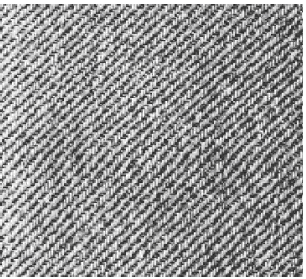
\includegraphics[width=5cm,]{Figures/chap1/direction.png}
&
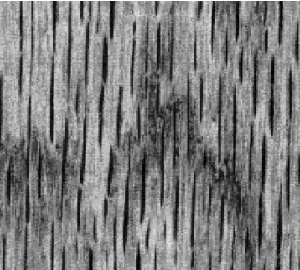
\includegraphics[width=5cm,]{Figures/chap1/directionel1.png}
&
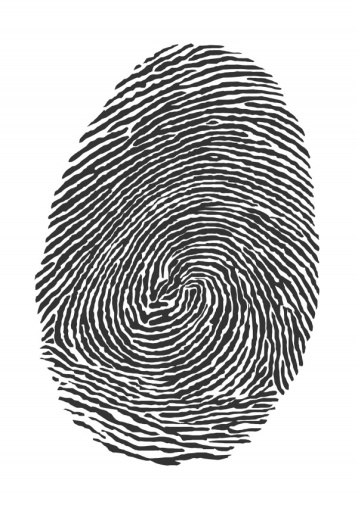
\includegraphics[width=3.5cm,]{Figures/chap1/directionel2.png}\\

\end{tabular}
\caption[textureDirex]{Textures directionnelles}
\end{figure}              


\indent Les textures directionnelles [Figure 1.5] ne sont pas forcément aléatoires et ne présentent pas d’éléments structurants de base.
On peut les décrire de manière générale comme étant des textures  présentant des structures orientées selon une direction privilégiée.
Les textures directionnelles se caractérisent soit par leur orientation globale, soit par un champ d’orientations locales. par exemple la texture de gauche de la figure 1.5 laisse apparaître des lignes obliques, et celle au milieu possède des lignes verticales.
Dans les textures directionnelles réelles, le champ d’orientation n’est en effet pas toujours uniforme comme la texture de droite de la figure 1.5.


\indent Les différentes catégories de textures qui ont été présenté nous montrent qu’il est difficile de donner une définition "universelle" de la texture. Cependant, on peut décrire le type de la texture selon la distribution et les relations entre les pixels qui la forment.\\

\indent Nous allons nous approfondir sur l’approche statistique étant donné qu’elle sera celle qu’on implémentera dans nôtre étude.
Plus précisément, nous étudirons la méthode suivante dite \textbf{motif binaire local}.


%------------------------------------------------
%------ [3] MOTIFS BINAIRE LOCAL (LBP) ----------
%------------------------------------------------

\section{Motif binaire local (LBP-Local Binary Pattern)}
\indent Cette caractéristique a été premièrement évoqué par Harwood [Har et.al 93] et a été utilisé après par Ojala et Pietikinen [Oja et.al 96, Oja and Pie 99].
La caractéristique LBP présente un énorme avantage grâce à sa simplicité de calcul et sa robustesse dans la détection de textures. Elle permet de décrire la texture suivant la configuration 

 locale des pixels.\\ 
\indent Le principe de calcul de la LBP basique (\textit{Basic Local Binary Pattern}) réalisé par Ojala [Oja et.al 02] est de comparer un pixel se trouvant au centre avec ces 8 voisins comme le montre la figure suivante :

\begin{figure}[H]
\centering
\begin{tabular}{ccc}
\centering

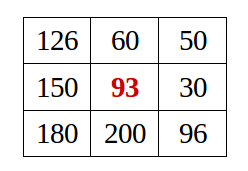
\includegraphics[width=5cm,height=3cm]{Figures/chap1/matrice1.png}
&
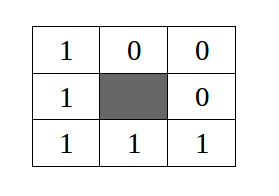
\includegraphics[width=5cm,height=3cm]{Figures/chap1/matrice2.png}
&
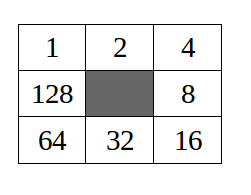
\includegraphics[width=5cm,height=3cm]{Figures/chap1/matrice3.png}\\
(a) & (b) & (c)\\
\end{tabular}
\caption[CalcMotif]{Calcul du motif binaire}
\end{figure}

\indent La matrice \textit{I} de la figure 1.6 (a) représente le niveau de gris d'un pixel au centre et de ses huit voisins. La matrice \textit{M} du \textit{motif} qui est représenté dans la figure 1.6 (b) est calculé comme suit :
$$M(i,j) = \left\{
\begin{array}{c c c}      
    1 & si & I(i,j)\geqslant g_{c}\\
    0 & sinon & 
\end{array}\right. $$
Où $I(i,j)$ est la valeur du niveau de gris des huit voisins, et $g_{c}$ qui est le niveau de gris du pixel central (en rouge), le résultat est alors affecté sous format binaire dans les $M(i,j)$.\\
En lisant les valeurs de $M(i,j)$ en commençant de la case qui se trouve en haut à gauche et en suivant l'ordre de rotation de l'aiguille d'une montre, on obtient le motif binaire \textit{m} suivant :

$$ m = 10001111 $$

Ce résultat sera ensuite converti en décimal et cela en multipliant chaque chiffre par les valeurs $P(i,j)$ case par case de la matrice de Poids de la [Figure 1.6](c), ce qui nous donne la valeur LBP du niveau de gris du pixel central qui est :

$$ LBP = 128+8+4+2+1 = 143 $$

La figure suivante montre la transformation LBP d'une image :

\begin{figure}[H]
	\centering
	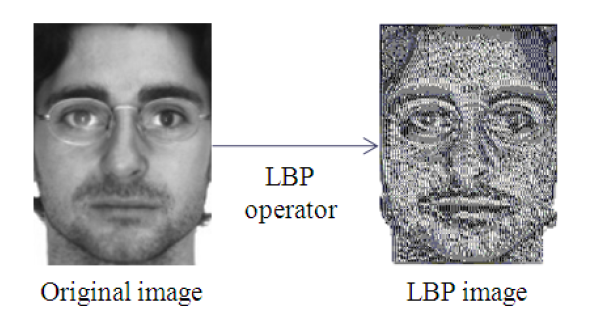
\includegraphics[width=9cm,]{Figures/chap1/transLBP.png}		
	\caption[transLBP]{Transformation LBP de l'image}
\end{figure}	


\indent Ojala [Oja et.al 02] a aussi définie une valeur "\textit{U}" qu'on appellera valeur de «\textit{transition}» qui sera égale au nombre de transitions de 0 vers 1 et de 1 vers 0 qu'on trouve dans la valeur du «\textit{motif binaire}» comme suit :\\

\begin{figure}[H]
	\centering
	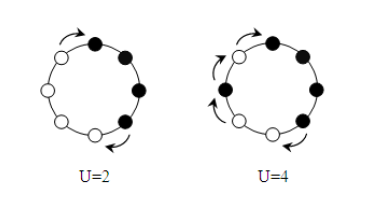
\includegraphics[width=8cm]{Figures/chap1/extractU.png}		
	\caption[extractU]{ Extraction du nombre U à partir du motif}
\end{figure}	

\indent En réalité, tous les «\textit{motifs}» (256) ne sont pas importants pour décrire une texture.
D'apres T. Menp [Men et.al 00], les motifs qui ont un nombre de transition $U=2$ et $U=0$, et qui sont appelés «\textit{uniform patterns}», représentent une information relative à des motifs réguliers d'une image, autrement dit une texture. Et donc, certaines zones d'intérêt tels des coins ou des bords peuvent être détectées par ce descripteur.
Ces motifs sont aussi plus résistants aux transformations géométriques telle que la rotation.
L’utilisation des 58 «\textit{uniform patterns}» suivants a été proposé :

\begin{figure}[H]
	\centering
	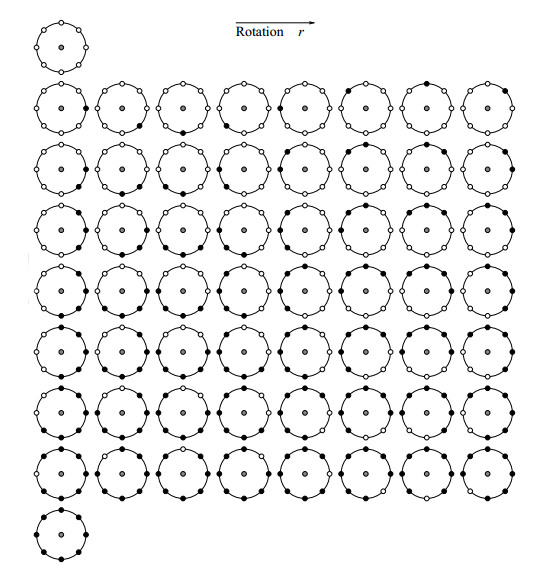
\includegraphics[height = 12cm]{Figures/chap1/uniforme.png}		
	\caption[uniforme]{ Les «\textit{uniform patterns}».}
\end{figure}	

\indent Pour étudier l’uniformité d'une texture, on construit un histogramme qui est composé de 59 valeurs qui sont les 58 «\textit{uniform patterns}» définis plus haut, plus une dernière valeur regroupant tous les «\textit{non uniform patterns}».\\

\begin{figure}[H]
\centering
\begin{tabular}{cc}
\centering

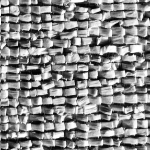
\includegraphics[width=3cm,height=6cm]{Figures/chap1/in1.png}
&
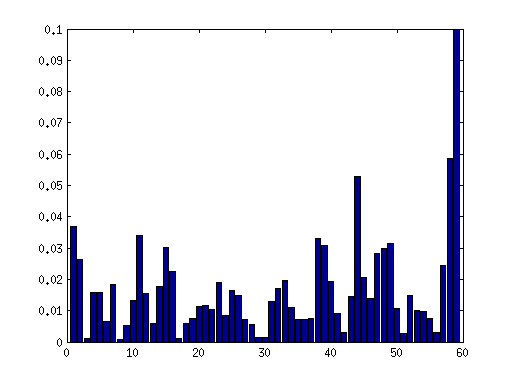
\includegraphics[width=6cm,height=6cm]{Figures/chap1/histo1.png}\\
(a) & (b) \\
\end{tabular}
\caption[histo]{Une texture et son histogramme LBP }
\end{figure}


\indent On compare deux histogrammes LBP de deux textures selon un pourcentage de ressemblance qu'on appellera «\textit{seuil}» ou encore «\textit{Threshold}».On pourra ainsi dire si ces deux textures représentent la même texture ou bien non grâce à cette valeur. 

\indent La caractéristique LBP qui utilisent ce genre d'histogramme est noté en tant que $LBP^{u2}$. Cette notation est du au fait qu'elle se base sur les «\textit{uniform patterns}» qui ont un $U \leq 2$, par la suite, on notera la $LBP^{u2}$ en tant que LBP.

\subsection{LBP et le niveau de gris}
\indent L'un des avantages de la LBP est sa robustesse vis à vis du changements monotones du niveau de gris. Ainsi, si on augmente ou diminue le niveau de gris de chaque pixel d'une image d'une même valeur $x$, cela n'affectera pas l'histogramme LBP créée. Cet avantage réside dans la manière de calcul du nouveau niveau de gris LBP d'un pixel.\\
\indent Soit un pixel $P$ qui va avoir une nouvelle valeur modifié par $x$, il sera comparé avec ses voisins $V_{i}$ (sachant que ses voisins sont aussi affecté par la valeur $x$) et on sait que :
\begin{center}
si $P > V_{i}$ alors $P + x > V_{i} + x $
\end{center}
\indent Et comme la comparaison n'a pas changé, alors la nouvelle valeur de niveau de gris du pixel centrale restera toujours la même, comme le montre la figure 1.10.\

\begin{figure}[H]
\centering
\begin{tabular}{cc}
\centering

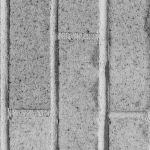
\includegraphics[width=3cm]{Figures/chap1/p1.png}
&
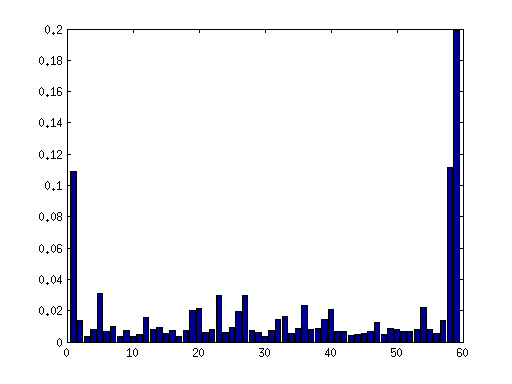
\includegraphics[width=6cm]{Figures/chap1/histcomp1.png}\\

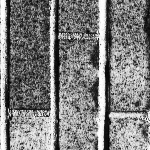
\includegraphics[width=3cm]{Figures/chap1/p2.png}
&
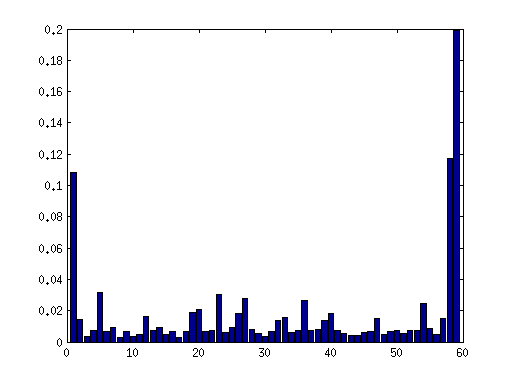
\includegraphics[width=6cm]{Figures/chap1/histcomp2.png}\\
\end{tabular}
\caption[comp]{Histogramme d'une texture subissant un changement monotone du niveau de gris}
\end{figure}


\subsection{Variantes de la LBP}
\indent Il existe d'autres variantes de la LBP qui divergent selon le nombre $P$ de voisins dans un rayon $R$, comme le montre la figure 1.11.\\
 
\begin{figure}[H]
\centering
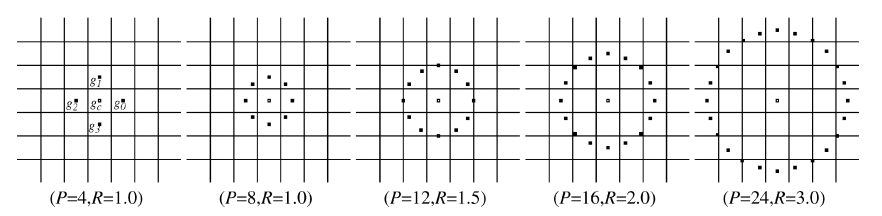
\includegraphics[width=15cm]{Figures/chap1/lbpvariantes.png}
\caption[lbpvar]{Variantes de la LBP}
\end{figure}

\indent Il a été noté que dans la LBP Basique ($P=8$ et $R=1$), le taux des «\textit{uniform patterns}» est presque de 90\%, alors que pour la LBP(16,2) ($P=16$ et $R=2$) ce taux ne dépassait pas les 70\%.[Oja et.al 02]
De ce fait, on se basera sur la LBP Basique qui offre une meilleure détection des textures.


\section{Conclusion}

\indent Dans ce chapitre nous avons décris la texture et ses différents types. Nous constatons que malgré le fait qu'il n'existe à priori toujours pas de définition universelle de la texture, les méthodes de description structurelles restent largement les plus utilisés.\\
\indent Nous avons présenté le \textbf{Motif binaire local} qui est une caractéristique très populaire et récemment employée pour détecter des personnes et dans la reconnaissance faciale.
Dans le chapitre suivant, nous allons parler de son utilité dans notre travail.